\section{緒言}%===========================
エアシリンダは生産現場などに多く使われている.しかし,長いストロークを持ちつつも,コンパクトに使用するような場合には適合しない.よって,十分にストロークがありつつも,設置しやすい直動アクチュエータが求められている.
\par
そこで,曲げられるエアシリンダを提案する.本研究では曲げられるエアシリンダを"細径柔軟エアシリンダ"と呼ぶ.図\ref{Small diameter flexible air cylinder}に細径柔軟エアシリンダを示す.細径柔軟エアシリンダは柔らかい素材で構成されている.そのため,曲がった状態で配置・動作し,高ストロークを有しつつもコンパクトに設置することができる.しかし,細径柔軟エアシリンダは曲がった状態において,シリンダとロッドが接触する現象が起こる.本稿では,1つ目の内容として,シリンダを環状に巻き付けた状態における理論出力を導出し,実験値と比較する.
\par
細径柔軟エアシリンダ単体では出力が小さいという課題がある.そこで,細径柔軟エアシリンダを束ねた"エアシリンダ型人工筋肉"を提案する.図\ref{artificial muscle}にエアシリンダ型人工筋肉を示す.エアシリンダ型人工筋肉は細径柔軟エアシリンダを7本束ねた構造である.束ねた構造により柔軟性と高出力化の両方を持つ.2つ目の内容として,エアシリンダ型人工筋肉における印可圧力と出力特性とステップ応答性を測定し,束ねた状態において動作可能か確認する.
\par
3つ目の内容として,細径柔軟エアシリンダを機械要素として使用する際の制御特性について確認を行う.細径柔軟エアシリンダを揺動アームの機械要素とし,アームの角度制御とアーム先端のコンプライアンス制御を行い,制御性について評価を行う.
これら3つの内容を踏まえて,細径柔軟エアシリンダ及びエアシリンダ型人工筋肉が機械要素としてどのように取り扱うかを確認する.
% 細径柔軟エアシリンダの基礎特性,細径エアシリンダを束ねた構造の基礎特性とステップ応答性,曲がった状態のエアシリンダの理論と実験,エアシリンダ型人工筋肉を取り付けた揺動アームの位置制御とコンプライアンス制御

% 1.曲がった細径柔軟エアシリンダの出力の理論化と実験値の比較
% 2.エアシリンダ型人工筋肉の提案とその出力特性
% 3.揺動アームの制御
\begin{figure}[t]
  \centering
  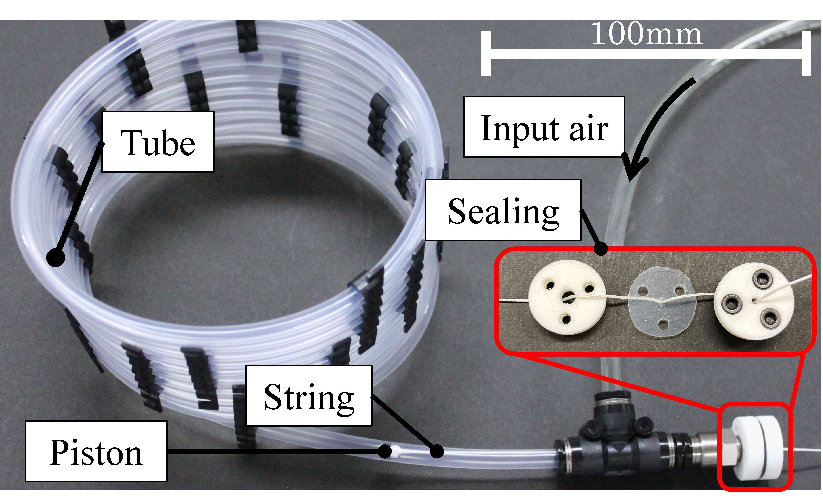
\includegraphics[width=85mm]{_pdf/細径柔軟エアシリンダ-1本.pdf}
  \caption{Small diameter flexible air cylinder}
  \label{Small diameter flexible air cylinder}
\end{figure}

\begin{figure}[t]
  \centering
  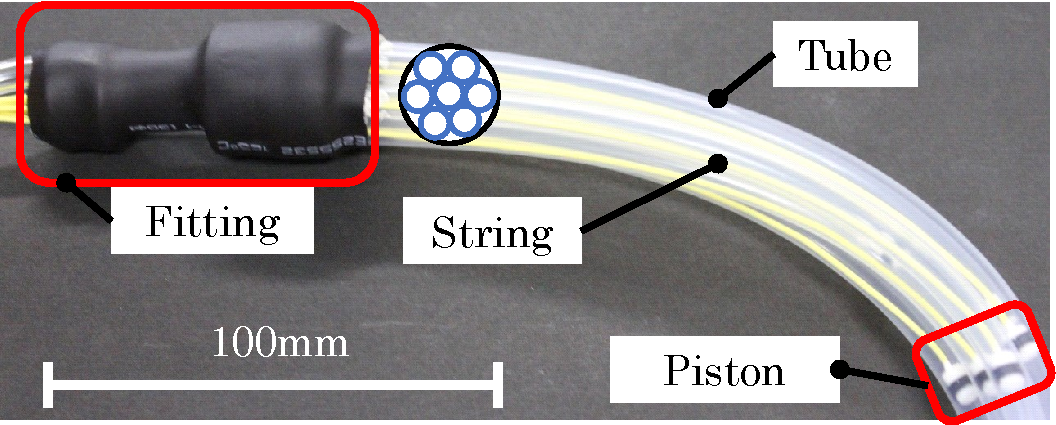
\includegraphics[width=85mm]{_pdf/紹介-エアシリンダ型人工筋肉.pdf}
  \caption{Air cylinder type artificial muscle}
  \label{artificial muscle}
\end{figure}

\section{環状に曲がった細径柔軟エアシリンダの理論出力}%-----------
\subsection{構造}%-----------
\begin{comment}
本研究で取り扱うエアシリンダ型人工筋肉とフィッティグの構造を図1に示す.問題の簡単化のためにシリンダ及びロッドの本数を1本とする.シリンダ部分は柔軟チューブ(ニチアス株式会社,材質:ナフロン\textregistered,内外径:$\SI{5}{mm}$, $\SI{6}{mm}$,最小曲げ半径:$\SI{35}{mm}$)である.ロッド部分は紐(ハヤミ工産株式会社,材質:イザナス®,線形:$\SI{0.60}{mm}$,破断強度:$\SI{360}{N}$,破断伸度:$\SI{5.5}{N}$)である.ピストンは2枚のフッ素ゴムリングを2枚のPLA樹脂部品で挟み込む構造である.シール部はゴムシート(材質:NBR,厚さ:1 mm,硬度:70 °(タイプA))である.ゴムシートに穴をあけてロッドを通している.ロッドを通したゴムシートを2つのプラスチック部品をボルトにより挟み込む.
\end{comment}
\subsection{理論出力の導出}%-----------

\subsection{理論値と実験値の比較}%-----------


\section{エアシリンダ型人工筋肉}
\subsection{構造と動作原理}
\begin{comment}
試作したエアシリンダ型人工筋肉を図\ref{artificial muscle}に示す.構造は,上述の細径柔軟エアシリンダを最密となるように$n$=7本配置したものである.フィッティングの内部構造を図\ref{fitting}に示す.内部は2つの部品(図中:赤,白色部品)に分かれており,それぞれ紐シール部(赤色)とシリンダシール部(白色)である.紐シール部は7個のピストンから伸びる紐が通るPTFEチューブ(中興化成工業株式会社,内外径:$\SI{1}{mm}$, $\SI{3}{mm}$,長さ:$\SI{4}{mm}$)をPLA樹脂部品に圧入している.シリンダシール部は7本のナフロン\textregistered チューブ(ニチアス株式会社,内外径:$\SI{5}{mm}$, $\SI{6}{mm}$,最小曲げ半径:$\SI{35}{mm}$)を挿入できるPLA樹脂部品を使用する.また,紐シール部に圧力印加用のチューブを挿入の後,接着している.シリンダシール部は2つのPLA樹脂部品から構成されており,目地剤(セメダイン株式会社,シリコーン系シーリング材8060プロ)を充填するための空間を設けるような構造である.紐シール部とシリンダシール部の端面に上述のねじ剤を塗布し,部品を覆うように熱収縮チューブ(モノタロウ,材質:ポリオレフィン樹脂,内径:収縮前$31.5\pm\SI{1.0}{mm}$,収縮後$\SI{15}{mm}$)を被せる.動作原理は上述の細径柔軟エアシリンダと同じではあるが,それらを束ねたことによって紐(ロッド)が7本出てしまうが,7本の紐を先端で結ぶことによって7本の細径柔軟エアシリンダの出力をまとめる.
\end{comment}

%なぜ太い1本ではなく,束ねるのか(断面二次モーメントから説明する).出力面積の観点では,束ねた方が不利になる.しかし,柔軟性を向上させるには束ねた方がよいことを説明する.また,1本1本のエアシリンダの出力特性が異なる.よって,束ねることによってそのばらつきを抑え,全体としての出力を担保することを説明する.太い1本の場合との比較を理論的な観点から説明すべき.製作方法についても言及すべき.エア漏れのことととか(これは実験結果から説明するほうがよいのか).

\subsection{印加圧力-出力特性}%-----------
\begin{comment}
図\ref{Output of artificial muscle}に曲率半径$r_a=\SI{100}{mm}$と曲率を有しない場合(曲率半径$r_a=\infty$)の2パターンにおける,細径柔軟エアシリンダの印加圧力に対する静的な出力の関係を示す.測定は計5回行い,それらの平均をプロットする.また,各測定の出力の最大最小値をエラーバーとして示す.図\ref{Output of artificial muscle}より,曲率半径$r_a=\SI{100}{mm}$と$\infty$の2パターンとも印加圧力に対して出力が比例して増加していることがわかる.また,細径柔軟エアシリンダを$n$=7本束ねたことによって印加圧力$P=\SI{300}{kPa}$における細径柔軟エアシリンダの出力と比較し曲率半径$r_a=\infty$の時は5.6倍,曲率半径$r_a=\SI{100}{mm}$の時は5.5倍に増加していることがわかる.しかし,束ねた本数$n$=7倍に出力が増加していないのは,紐シール部からのエア漏れによってピストンにかかる圧力が印加圧力よりも小さくなったためだと考えられる.曲率半径$r_a=\SI{100}{mm}$と$\infty$を比較すると,わずかではあるが曲率半径$r_a=\SI{100}{mm}$の出力が小さいことがわかる.細径柔軟エアシリンダの出力と同様にシリンダの湾曲に伴って,シリンダとピストンの摩擦損失が増加し,出力が小さくなったと考えられる.これらの結果より,細径柔軟エアシリンダを$n$本束ねた場合においても,出力がおおよそ$n$倍になることがわかった.よって,細径柔軟エアシリンダを束ねることによって曲げ剛性を抑えつつも,出力が増加することを確認した.
\begin{figure}[t]
  \centering
  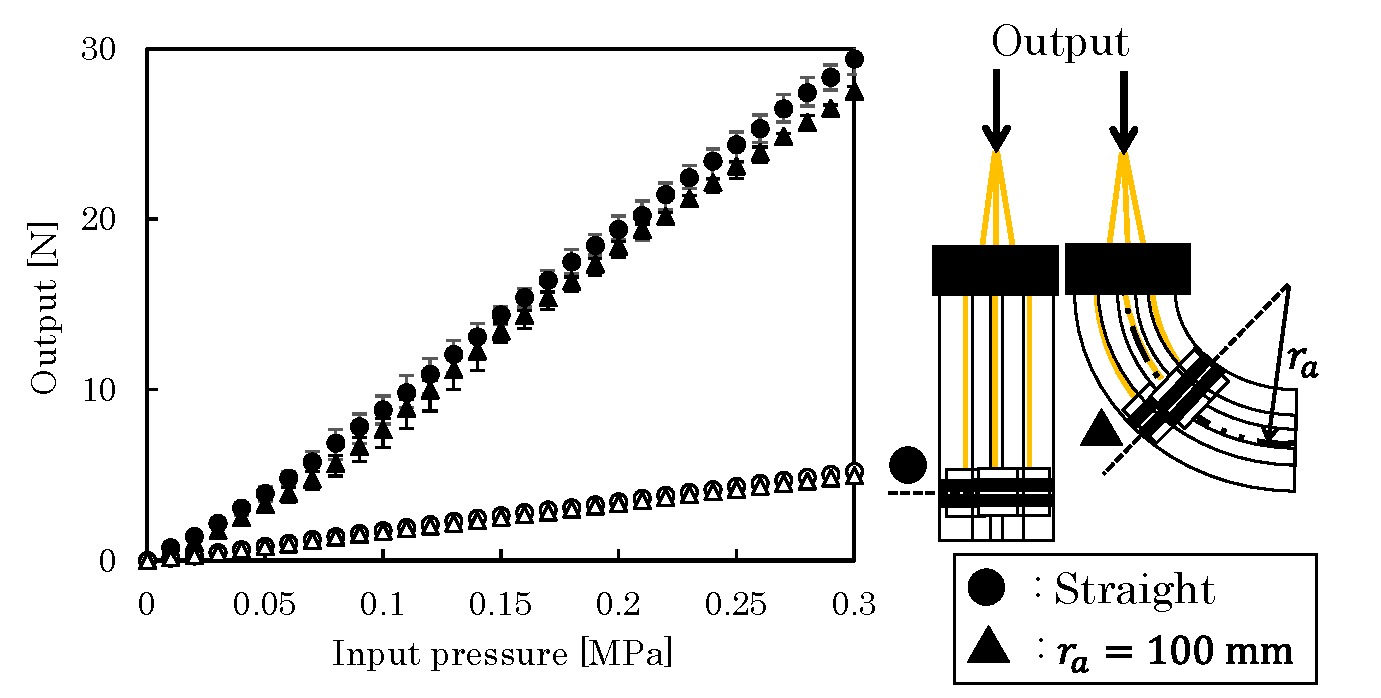
\includegraphics[width=85mm]{_pdf/出力特性-エアシリンダ型人工筋肉.pdf}
  \caption{Output of an air cylinder type artificial muscle}
  \label{Output of artificial muscle}
\end{figure}
\end{comment}

\subsection{応答性}%-----------
\begin{comment}
エアシリンダ型人工筋肉に圧力を印加した時の応答性がどの程度であるか測定を行う.本実験では,エアシリンダ型人工筋肉が真っすぐな状態と一部分が湾曲した状態の2パターンの測定を行う.特に,湾曲した部分では出力が低下するため応答性がどの程度減少するのか確認を行う.本実験では電磁弁のオン・オフをステップ入力とし,エアシリンダ型人工筋肉の圧力とピストン移動距離のステップ応答を確認する.
\subsubsection{実験方法}
使用する実験装置を側面から見たものを図\ref{Experimental device of step response}に示す.エアシリンダ型人工筋肉のフィッティングとシリンダ末端は実験装置に固定する.ロッドにはプーリを介し,地面と垂直になるように垂らし,先端に錘を接続する.空圧機器の構成は,コンプレッサ(圧縮空気入り口)→圧力調節器→電磁弁(SMC,型番:SY113-5L-M3)→圧力計→エアシリンダ型人工筋肉の順に接続する.
\par
エアシリンダ型人工筋肉には電磁弁のオン・オフをステップ入力とし,圧力センサで印加圧力を測定する.また,錘の移動距離を画像処理で測定する.なお,エアシリンダ型人工筋肉には電磁弁を解放した時,圧力計において$P_t=\SI{220}{kPa}$となるように圧力調節器で調節を行う.錘は$\SI{1000}{g}$のものを使用する.
\par
本実験では,エアシリンダ型人工筋肉のシリンダが真っすぐな状態(経路A)と一部分に曲率半径$r_a=\SI{100}{mm}$の湾曲を設けた状態(経路B)の2パターンの測定を行う.経路Aの長さ$L_A=\SI{330}{mm}$とする.経路Bは湾曲部の長さ$L_{B1}=\SI{157}{mm}$と湾曲していない箇所の長さ$L_{B2}=\SI{173}{mm}$の合計長さ$L_{B1}+L_{B2}=L_B=\SI{330}{mm}$とする.

\begin{figure}[t]
  \centering
  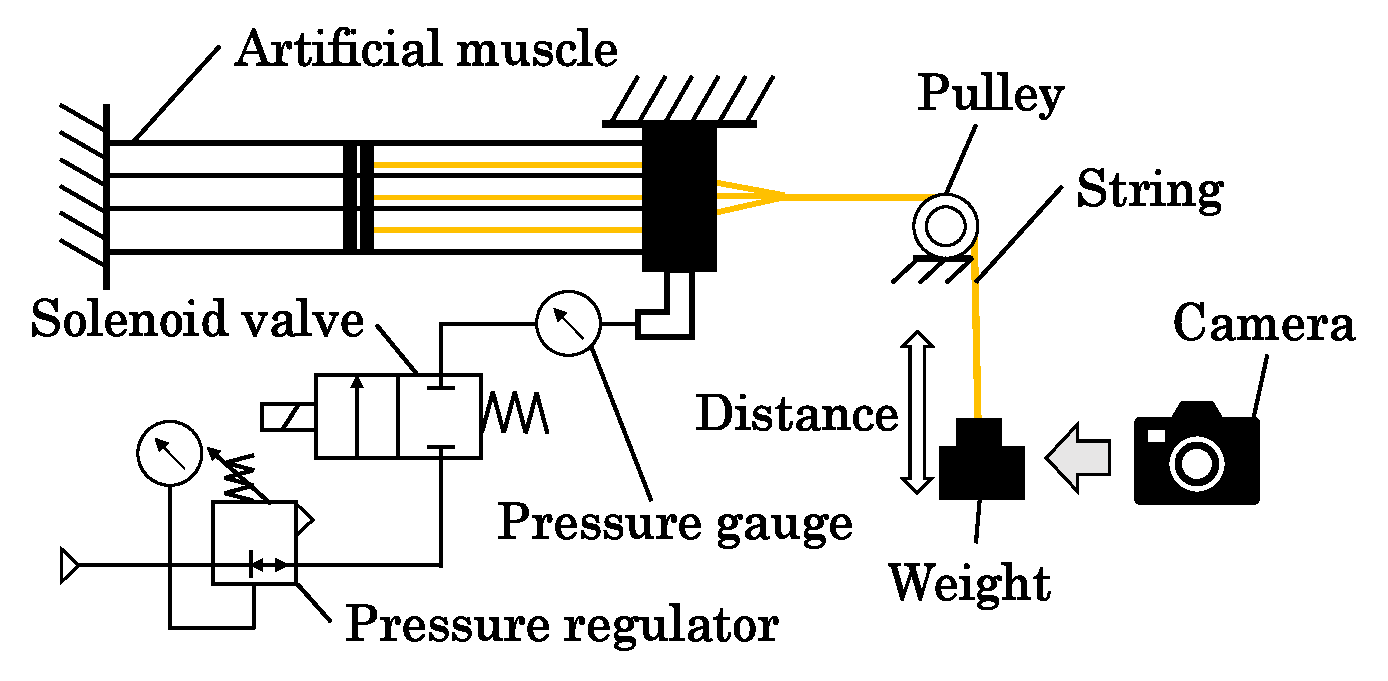
\includegraphics[width=85mm]{_pdf/実験装置-ステップ応答.pdf}
  \caption{Experimental device of step response}
  \label{Experimental device of step response}
\end{figure}

\subsubsection{実験結果・考察}%-----------
図\ref{Step response of input pressure}に経路Aと経路Bにおける印加圧力のステップ応答を示す.また,図\ref{Step response of distance}に経路Aと経路Bにおける錘の移動距離のステップ応答を示す.なお,測定は経路A,経路Bともに10回行い,それらの平均をプロットする.また,各測定の印加圧力,錘の移動距離の標準偏差をエラーバーとして示す.図\ref{Step response of input pressure}より,経路A,経路Bともにステップ入力から$\SI{0.5}{s}$経過した後,目標圧力$P_t=\SI{220}{kPa}$に達している.ステップ入力をオフにしたときの応答は経路A,経路Bともに$\SI{0.2}{s}$で下がりきっている.立ち上がる時の目標圧力$P_t$の$\SI{60}{\%}$付近で印加圧力が減少している箇所が確認できる.図\ref{Step response of distance}より,目標距離に達した時と図\ref{Step response of input pressure}の圧力減少の箇所が同一であるとわかる.よって,エアシリンダ型人工筋肉のピストンが急に停止することが,立ち上がり途中の圧力減少に影響すると考えられる.ピストンが急に停止すると,シリンダ内の体積膨張が停止する.そして,印加した空気の行き場がなくなり紐シール部からのエア漏れが急速に起こることによって圧力が減少すると考えられる.図\ref{Step response of input pressure}の経路Aと経路Bを比較すると,わずかではあるが経路Bが経路Aに対して立ち上がりが遅れている.しかし,遅れ時間は$\SI{0.1}{s}$であり湾曲を設けた場合でも立ち上がりには大きく影響しないと考えられる.図\ref{Step response of distance}の経路Aと経路Bを比較すると,目標距離$D_t=\SI{330}{mm}$に立ち上がるまで経路Bが経路Aに対してわずかではあるが遅れている.印加圧力のステップ応答と同様に,経路Aと経路Bに大きな差はなく湾曲による影響は少ないと考えられる.図\ref{Step response of distance}のステップ入力をオフにしたときの応答は$\SI{0.5}{s}$で初期位置に戻っていることがわかる.図\ref{Step response of input pressure}より立下りの際に印加圧力が瞬時に大気圧に戻っているため錘の位置も瞬時に戻ったと考えられる.以上の結果より,湾曲をもうけた経路とまっすぐな経路の動的な特性には大きな差がないことがわかった.また,経路A,経路Bどちらにおいても立ち上がり,立ち下がりは良好であることを確認した.
\begin{figure}[t]
  \centering
  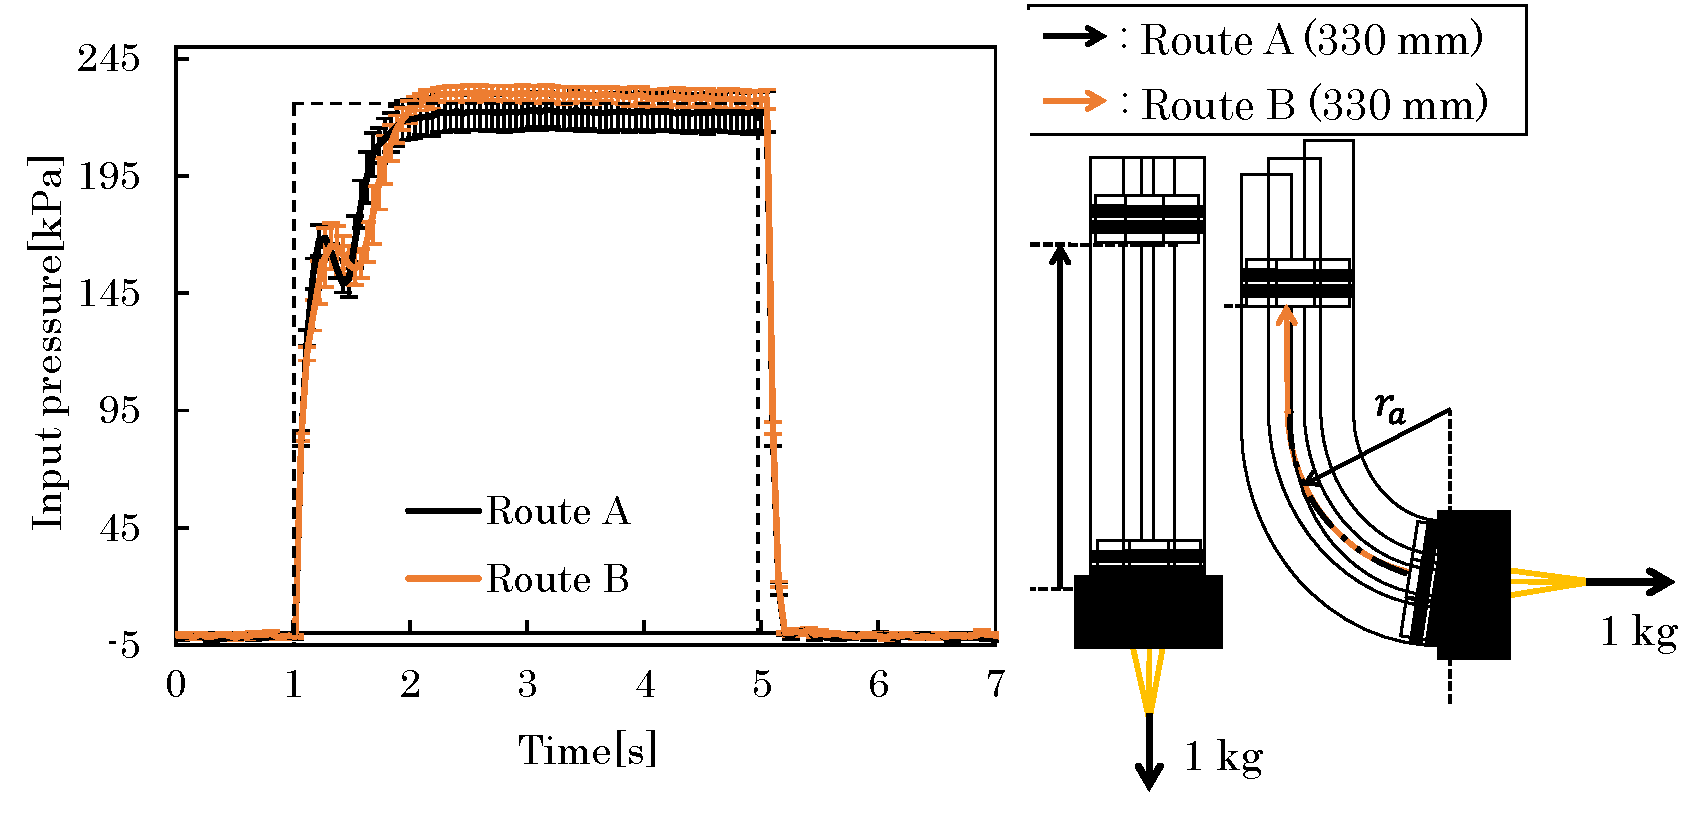
\includegraphics[width=85mm]{_pdf/ステップ応答-印加圧力.pdf}
  \caption{Step response of input pressure}
  \label{Step response of input pressure}
\end{figure}

\begin{figure}[t]
  \centering
  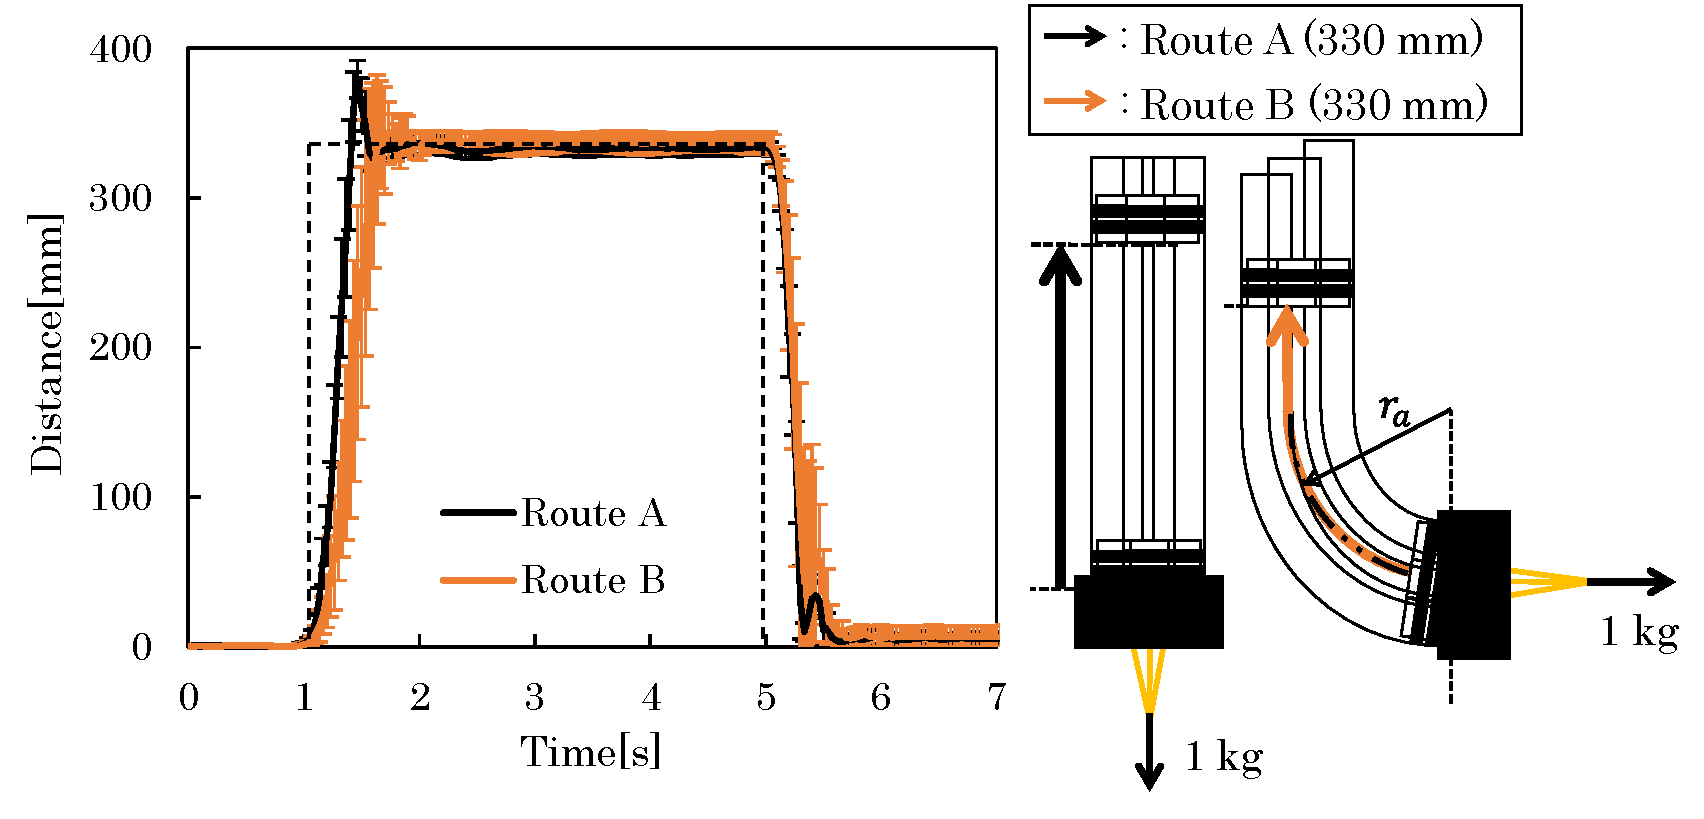
\includegraphics[width=85mm]{_pdf/ステップ応答-移動距離.pdf}
  \caption{Step response of distance}
  \label{Step response of distance}
\end{figure}
\end{comment}

\section{細径柔軟エアシリンダの制御性}%-----------
\subsection{揺動アームの構造}
\subsection{揺動アームの角度制御}
\subsection{アーム先端のコンプライアンス制御}

\section{結言}%-----------
\begin{comment}
従来の高剛性・精密につくられるエアシリンダは,ストロークを長くするとそれに伴ってエアシリンダ自体が大型化してしまう.大型化に伴って,限られたスペースにエアシリンダを配置するために,適切な配置方法の検討が必要になるという課題がある.よって,本研究は曲げた状態で配置・動作可能な柔軟エアシリンダを提案した.まず,細径柔軟エアシリンダを提案し,試作を行った.印加圧力-出力特性より湾曲に伴う出力低下が小さいことがわかった.しかし,細径柔軟エアシリンダ1本では印加圧力$P=\SI{300}{kPa}$における出力が$\SI{5}{N}$と小さいため,それらを$n$=7本束ねた構造のエアシリンダ型人工筋肉を提案した.印加圧力-出力特性より,細径柔軟エアシリンダと比較して,出力が曲率半径$r_a=\infty$の時は5.6倍,$r_a=\SI{100}{mm}$の時は5.5倍に増加することがわかった.また,曲率半径$r_a=\SI{100}{mm}$に湾曲させた場合において曲率半径$r_a=\infty$と比較し出力の低下が小さいことがわかった.また,ステップ応答より,ストローク$S=\SI{300}{mm}$,印加圧力$P=\SI{220}{kPa}$,シリンダが真っすぐな状態の経路Aの立ち上がり時間が$\SI{0.5}{s}$であることがわかった.また,曲率半径$r_a=\SI{100}{mm}$を有した経路Bにおいても立ち上がり時間は$\SI{0.6}{s}$となり,シリンダが真っすぐな経路Aと比較して$\SI{0.1}{s}$遅くなることがわかった.これらの結果より,湾曲した場合でも,出力が大きく低下することがないことと,立ち上がり時間も大幅に遅くなることはないことがわかった.上記の結果より,エアシリンダ型人工筋肉は曲げた状態でも配置・動作ができるということを確認した.
\end{comment}
